\begin{pastexam}[label={px:ncku-109-prog-03}]{成大資訊聯招 109 學年度 資料結構第 3 題}
（計算）

Consider the following graph:

\begin{center}
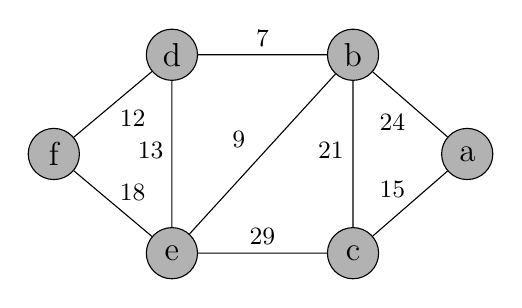
\begin{tikzpicture}[x=1cm,y=-0.9cm,v/.style={circle,draw,fill=black!30,inner sep=0pt,minimum size=6.5mm,font=\large},w/.style={font=\small,inner sep=1pt}]
\node[v] (d) at (2.4,0.95) {d}; \node[v] (b) at (4.7,0.95) {b};
\node[v] (f) at (0.9,2.35) {f}; \node[v] (a) at (6.15,2.35) {a};
\node[v] (e) at (2.4,3.75) {e}; \node[v] (c) at (4.7,3.75) {c};
\draw (f)--(d) (d)--(b) (d)--(e) (f)--(e) (e)--(b) (b)--(c) (b)--(a) (c)--(a) (e)--(c);
\node[w] at (1.9,1.85) {12}; \node[w] at (3.55,0.72) {7}; \node[w] at (2.13,2.3) {13}; \node[w] at (1.9,2.9) {18};
\node[w] at (3.25,2.15) {9}; \node[w] at (4.42,2.3) {21}; \node[w] at (5.2,1.9) {24}; \node[w] at (5.2,2.85) {15}; \node[w] at (3.55,3.52) {29};
\end{tikzpicture}
\end{center}

Compute minimum cost and construct minimum spanning tree. (10\%)
\end{pastexam}

\begin{pastsoln}
答案：最小成本是 $64$，最小生成樹的邊是 $db\,(7)$、$eb\,(9)$、$fd\,(12)$、$ca\,(15)$、
$bc\,(21)$。

圖有 $6$ 個頂點、$9$ 條邊：$fd = 12$、$db = 7$、$de = 13$、$fe = 18$、$eb = 9$、$bc = 21$、
$ba = 24$、$ca = 15$、$ec = 29$。 用 Kruskal 演算法（資結書第~24.2~節），邊依權重由小到大
看，兩端已經在同一棵樹裡就跳過：
\begin{center}
\begin{tabular}{clll}
\toprule
權重 & 邊 & 動作 & 之後的元件 \\
\midrule
7 & $db$ & 加入 & $\{b, d\}$ \\
9 & $eb$ & 加入 & $\{b, d, e\}$ \\
12 & $fd$ & 加入 & $\{b, d, e, f\}$ \\
13 & $de$ & 跳過（$d$、$e$ 已經相連） & \\
15 & $ca$ & 加入 & $\{b, d, e, f\}$、$\{a, c\}$ \\
18 & $fe$ & 跳過（$f$、$e$ 已經相連） & \\
21 & $bc$ & 加入，兩個元件合併 & $\{a, b, c, d, e, f\}$ \\
\bottomrule
\end{tabular}
\end{center}
加入第 $5 = 6 - 1$ 條邊時已經連成一棵樹，$ba = 24$、$ec = 29$ 不用再看（看了也會跳過）。
總成本
\[
7 + 9 + 12 + 15 + 21 = 64.
\]
九條邊的權重都不同，所以最小生成樹只有這一棵（資結書定理~24.4）。 圖中粗線是最小生成樹：

\begin{center}
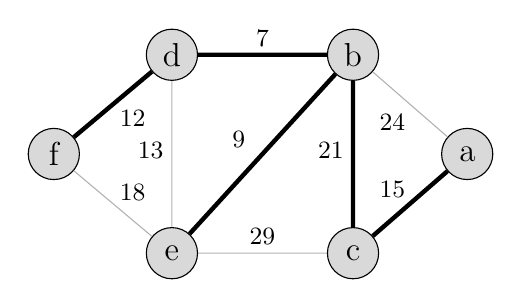
\begin{tikzpicture}[x=1cm,y=-0.9cm,v/.style={circle,draw,fill=black!15,inner sep=0pt,minimum size=6.5mm,font=\large},w/.style={font=\small,inner sep=1pt}]
\node[v] (d) at (2.4,0.95) {d}; \node[v] (b) at (4.7,0.95) {b};
\node[v] (f) at (0.9,2.35) {f}; \node[v] (a) at (6.15,2.35) {a};
\node[v] (e) at (2.4,3.75) {e}; \node[v] (c) at (4.7,3.75) {c};
\draw[black!30] (d)--(e) (f)--(e) (b)--(a) (e)--(c);
\draw[line width=1.6pt] (f)--(d) (d)--(b) (e)--(b) (b)--(c) (c)--(a);
\node[w] at (1.9,1.85) {12}; \node[w] at (3.55,0.72) {7}; \node[w] at (2.13,2.3) {13}; \node[w] at (1.9,2.9) {18};
\node[w] at (3.25,2.15) {9}; \node[w] at (4.42,2.3) {21}; \node[w] at (5.2,1.9) {24}; \node[w] at (5.2,2.85) {15}; \node[w] at (3.55,3.52) {29};
\end{tikzpicture}
\end{center}

用 Prim 演算法從 $a$ 開始也得到同一棵樹，依序加入 $ca\,(15)$、$bc\,(21)$、$db\,(7)$、
$eb\,(9)$、$fd\,(12)$。
\end{pastsoln}
